\setcounter{section}{8}
\section{Nyquist-Diagramm (Stabilität)}
\begin{tcolorbox}[colback=white!10!white,
                  colframe=blue!50!white,
                  title=Konstruktionsregeln Nyquist-Diagramm]
    \begin{enumerate}
    \item Betrag und Phase für mehrere Punkte aus dem Amplitudengang und 
        Phasengang des Bode-Diagramms ablesen. 
    \item Die Länge des Zeigers $10^{\frac{A_{dB}(\omega)}{20}}$ zum Nyquist-Plot ist der 
        Wert im Amplitudengang.
    \item Der Winkel des Zeigers ist $\varphi(\omega)$
    \item Für $\omega = 0^{\circ}$ bis $\omega = \infty$
    \item Instabil, wenn der Nyquist-Plot die $-1$ umschließt.
\end{enumerate}
\begin{figure}[H]
    \begin{subfigure}{0.5\linewidth}
        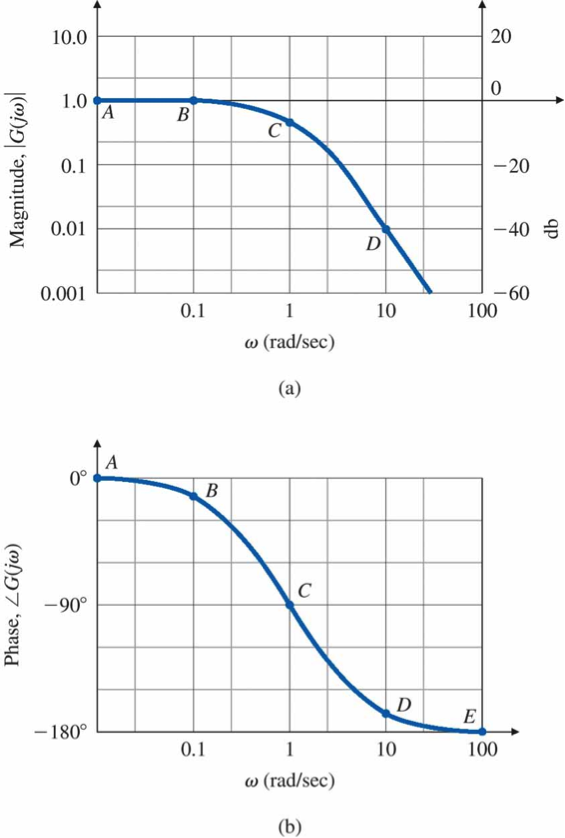
\includegraphics[width=\linewidth]{images/nyquist2}
    \end{subfigure}
    \begin{minipage}{0.45\linewidth}
        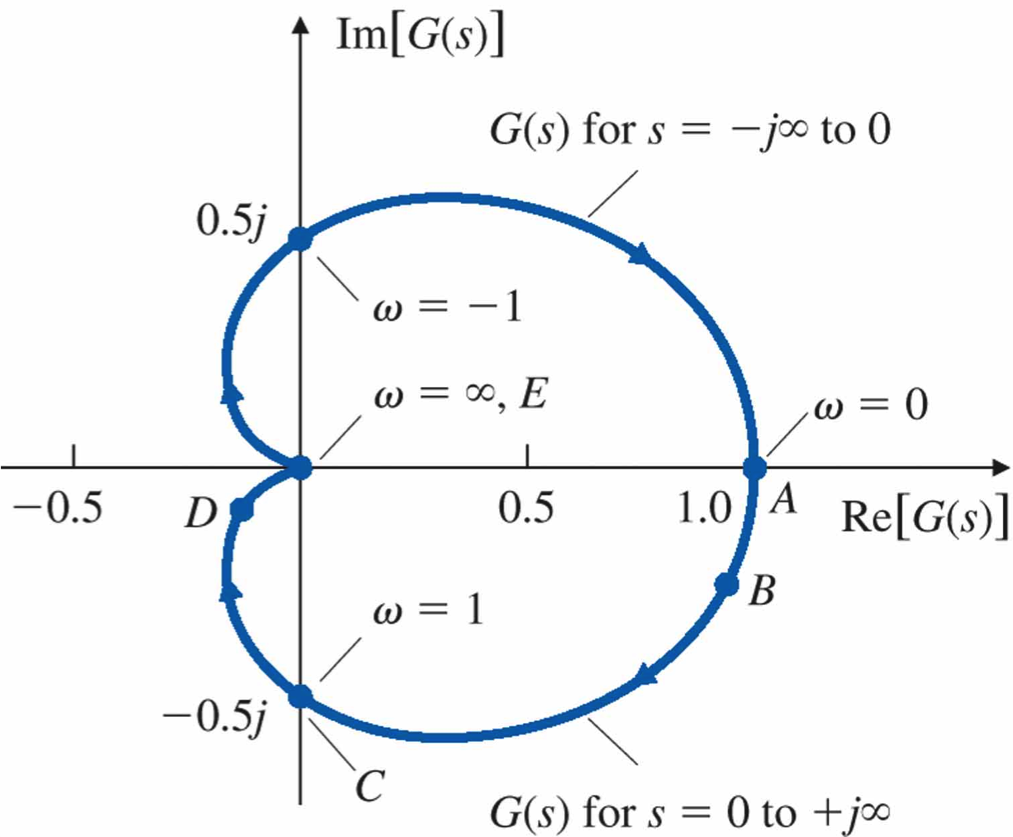
\includegraphics[width=\linewidth]{images/nyquist3}
    \end{minipage}
\end{figure}
\end{tcolorbox}

\begin{tcolorbox}[colback=white!10!white,
    colframe=green!30!black,
    title=Nyquist]
    \begin{figure}[H]
        \begin{subfigure}{0.5\linewidth}
            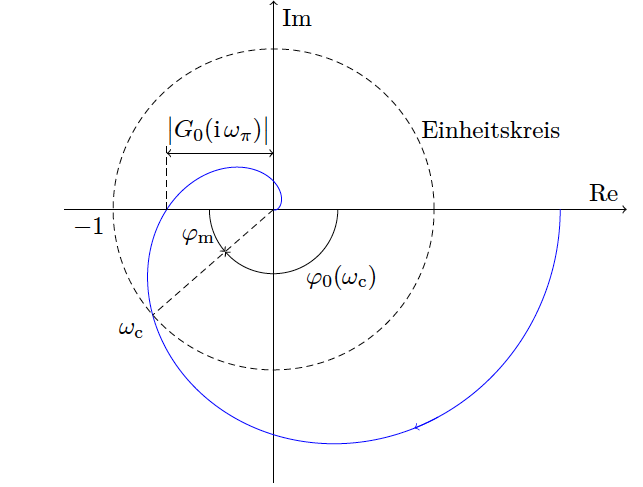
\includegraphics[width=\linewidth]{images/nyquist}
            \label{fig:nyquist}
        \end{subfigure}
        \begin{minipage}{0.45\linewidth}
            Amplituden-/ Betragsreserve 
            \begin{align*}
            &G_m = \frac{1}{|G_0(i\omega_\pi)|}\\
            & \omega_\pi = -180^{\circ}
            \end{align*}
            Phasenreserve ($\omega_c$ ist im Bode Diagramm, da wo Amplitudengang $0$dB schneidet):
            \begin{align*}
            &\phi_m = \pi + \phi(\omega_c)
            \end{align*}
        \end{minipage}
        Übliche Werte sind $G_m = 2,5 \ldots  10$ und $\phi_m = 30^{\circ} \dots 60^{\circ}  $. 
        
        Zur Stabilitätsanalyse kann man prüfen $|G_0(i\omega_\pi)| $ größer oder kleiner als 1 ist. 
    \end{figure}
    \tcblower
    \begin{figure}[H]\centering\begin{tikzpicture}
        \node(b2n) at (0,0) [
            inner sep=0pt,outer sep=0pt,anchor=north west
        ] {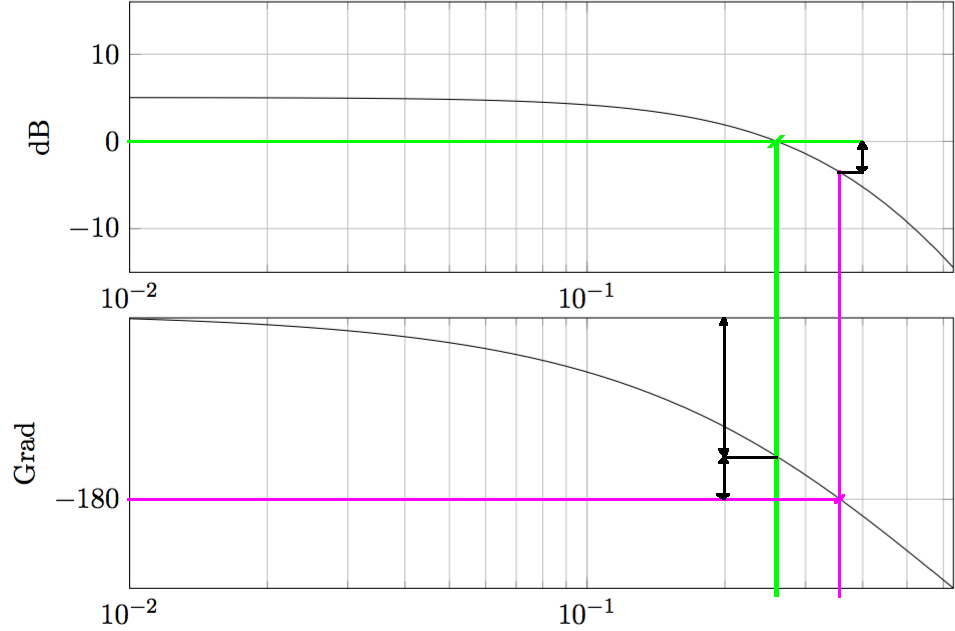
\includegraphics[width=\textwidth]{images/bode2nyquist1}};
        \node(omega-c) at (b2n.south) [
            inner sep=0pt,outer sep=0pt,anchor=south,
            yshift=0.01\textwidth,
            xshift=0.32\textwidth,
        ] {$\omega_c$};
        \node(phi-0) at (b2n.center) [
            inner sep=0pt,outer sep=0pt,anchor=north,
            yshift=-0.05\textwidth,
            xshift=0.23\textwidth,
        ] {$\varphi_0$};
        \node(phi-m) at (phi-0.south) [
            inner sep=0pt,outer sep=0pt,anchor=north,
            yshift=-0.085\textwidth,
        ] {$\varphi_m$};
        \node(omega-pi) at (b2n.south) [
            inner sep=0pt,outer sep=0pt,anchor=south,
            yshift=0.01\textwidth,
            xshift=0.39\textwidth,
        ] {$\omega_\pi$};
        \node(G-0) at (b2n.center) [
            inner sep=0pt,outer sep=0pt,anchor=north,
            yshift=0.22\textwidth,
            xshift=0.42\textwidth,
        ] {$G_0\left(i\omega_\pi\right)$};
        \end{tikzpicture}\end{figure}
    Mit $\varphi_m = \pi + \varphi_0\left(\omega_c\right)$ und
    $G_m = \frac{1}{\left|G_0\left(i\omega_\pi\right)\right|}$
\end{tcolorbox}

\begin{tcolorbox}[colback=white!10!white,colframe=red!60!black,title=Berechnung Betragsreserve aus G(s)]
     Gegeben ist eine Übertragungsfunktion:
     \begin{align*}
        &G(s) = \frac{10}{s^3+11s^2+11s+10}
     \end{align*}
     $j\omega$-Einsetzen  - und auf die untere Form bringen:
     
     Umformen auf
     \begin{align*}
         G(j\omega) &= \frac{10}{\text{Re} + j\omega \text{Im}} = \\
         &=\frac{10}{(-11\omega^2+10)+i\omega (11-\omega^2)}\\
         \tan(-\pi) &= 0 = \frac{\omega_{\pi}(11-\omega_{\pi}^2)}{ \omega_{\pi}^2 +10}\\
     \omega_{\pi} &= \sqrt{11}\\
     G(i\omega_{\pi}) &= \frac{10}{-111}  = 20,9 \text{dB}
     \end{align*}
\end{tcolorbox}
